\section{Diverse}

  {\bf Bias:} When a user are able to make their own password, the password that is created is often influenced by different biases.  When we are talking about a bias in terms of passwords, a the password making process can be influenced by biases like the demography of a person or the visualization of the password scheme. 
    
  {\bf Mobile Devices: } When talking about graphical password, they are not widely adopted on mobile devices. There are still some graphical passwords that are made for mobile devices, and this section will give a state-of-the art on graphical passwords for mobile devices.
  Our mobile devices are used for different authentication task. In the background theory, it was stated that we had mainly three different authentication schemes, e.g. ``something you know'', ``something you have'', and ``something you are''.
  As stated earlier, 

  {\bf Passwords in a business setting:} Passwords are not just used in our private life, but also a requirement in a critical concern from a business point of view where the use of authentication for corporate systems, mobile, and room codes plays a major role in normal day of work. In corporate systems users are often promt with the a notification forcing them to change the password in a specified time interval. The problem with this is that user already have problems remembering their passwords as is. A research group conducted a questionnaire survey in a large organization \cite{habits2}. The goal was to get a understanding of password habits in a business point of view. The results showed that the users were prompt with password change 7 times a year causing 68\% of the employees to re-use the same password with a minor change in order to still be able to remembering their passwords.

  Since the first graphical password schemes was proposed, it is not widely in use. One of the problems with graphical approaches are that they require more overhead in the authentication phase. Like text-based passwords the users can simply type their passwords, while many of the graphical passwords require to go through many steps, requiring the user to spend more time in the authentication phase. The graphical password schemes like Passface and grIDsure are some of the graphical password schemes with commercial interest, while on mobile devices graphical passwords are not widely adopted. There is a known problem with authentication on mobile devices because of the difficulty of typing on mobile keyboards, making authentication schemes using alternatives getting increased attention. Because of the difficulty of writing on mobile keyboards it highlights the importance of understanding the usability and security implications.


% \item To what extent can graphical elements like colors, shapes, and objects infuence the end-users choice of passwords?
% \item How is features describing the end-user picked, and how do the features relate to end-user's choice of passwords?
% \item Kan grafiske elementer påvirke brukerens valg av passord?
% \item Hvilke kjennetegn ved en person kan gi utslag på valg av passord?
% \item Hvordan skal innsamling av passord skjer for å ivareta datasamlingens pålitelighet?

% \item To what extent can we relate existing research on users choice of alphanumeric passwords to users choice of Android unlock patterns? 
% \item How should passwords from end-users be collected in order to preserve the reliability of the data? 
% \item In order to analyse collected Android unlock patterns, how much data is needed to be collected, and how should the diversity of the data look like?
% \item What kind of data should be included in the data model?
% \item How should the data model be designed in order to cover relevant data for the analysis of the collected data?  
% \item What are the status on research on mobile security?
% \item How should passwords from end-users be collected in order to preserve the reliability of the data? 


  {\bf Introduction}
  
  In todays society we're addicted to our mobile devices in our every day life. Mobile devices are not just a communication tool for calling and texting, but also an important tool for every day tasks like doing our work, reading mail, pay our bills and keeping up with our social life. Our whole life is contained in one device! When such a small device is so imortant, it makes it vurnerable. How do we secure it?
  %Information security have become a critical concern from a business point of view
  There are many different security tips for mobile devices, but the most imortant of them is locking your device with a password. There are many different password schemes, but the most commonly used password schemes are PINs, passphrases and graphical passwords.
  The interest in graphical passwords started by the assumption that pictures are easier to remember and more secure than words and numbers. Google's Android platform released the  functionality for Unlock Unlock Patterns in 2008. The Android Unlock pattern is a graphical password schemes that asks the user to make a pattern on a 3x3 grid by making a patten of connected nodes. Since its relese there have been a lot of discussion of its security, but few researchers have done a scientific reseach on this. The problem is not just the theoretical password space, but the password space in practice.
  In 2013 a research group conducted the first large-scale user study on Android Unlock Patterns \cite{Uellenbeck}. The outcome of the research was a analysis of 2900 collected Android Unlock Patterns. They found a lot of bias in the pattern making process cocluding that the schemes are less secure than its theoretical security.
  %Reasons for locking or not locking

  {\bf Motivasjon}

  - Fra empiriske boka kap 2: 
    * Test or disprove a theory
    * To come up with a better way
  - Paper til Markus.
  - Fortsette på studiet til Markus. 
  - Per Thorsheim sine studier på PIN koder
  - I dagens samfunn inneholder mobile enheter mer og mer sensitiv informasjon, 
    men våre kunnskaper om autentisering og sikkerhet henger ikke med i samme fart. 
  - Se sammengengen mellom personer og deres valg av mønstre
  - Se sammenheng mellom psykologi og teknologi/sikkerhet
    % Quote: “Somewhere, something incredible is waiting to be known.” 
    % ― Carl Sagan
    % “If you have built castles in the air, your work need not be lost; that is where they should be. Now put the foundations under them.” 
    %   ― Henry David Thoreau, Walden

  {\bf Background Theory}
  %  \section{Passphrase and PIN's vs. graphical passwords}
  %  \section{A password are more then just a password}

  %    If you take a walk in the street and ask a random person ``what is a password?'', 
  %    you probably get the aswer ``its letters and digits''. Passwords are so much more than just letter and digits. 

  %    Nowadays everything we do require you to keep this secret called a password. Your work, you're social life, 
  %    even you're private life is forcing you to keep track of passwords. How do you keep track of all of them?
  %    You probably keep the same password at many places. 
  %    \subsection{Theoretical Password Space}
  %    \subsection{Practical Password Space}

  %  \section{Relevant Data Collection Methods}
  %    In this section I will explore different methods for collecting data. It will give a brief summary of the 
  %    method as well as summary and discussion of the different methods at the end. 
  %    \subsection{Android Unlock Patterns Games}
  %    \subsection{Relevant User Studies}
  %    \subsection{Summary of Methods}
  %  \section{Information gathering}
  % \section{Psycology and passwords}
  % \section{Graphical passwords}
  % \section{Android Unlock Pattern}


  {\bf Environment in user study (OBS, DIREKTE HENTET FRA PAPER):} asked by security people in a security study to chose a secure password, people tend to overcompensate and choose rather complicated passwords. This behaviour is well known in psychology under the name ``priming'' and documented in several studies. All in all, this may lead users to choose stronger passwords than ones we would expect ``in the wild''.

  {\bf Introduksjon av noe slag:} In the litterature on graphical password it was found research with different focus. There have been published a lot of research that measures the usability of graphical passwords, but it still remains to look at the security of graphical passwords. However, there are not many researchers that have looked closer to the memorable password space and security of graphical password. As stated, mobile devices is a suited platform for graphical passwords, but there remains a lot of work here. The Android Unlock patterns is one of the graphical password schemes that are rapidly in use. As far as this study is familiar with, there is only one reaseach group that have published a large scale user study on the Android Unlock Patterns \cite{Ullenbeck}. One of the main challenges of working on graphical passwords is to be able to collect realiable user-chosen passwords. In contrast to text-based passwords were you can find lists of leaked passwords, this is unlikely to find for Android Unlock Patterns since they are stored in a centralized database. Passwords is something users dont give away easily, so how can we analyse user choice of password?  This study will design an experiment that will be conducted in the following spring. The experiment will collect data from users choices of patterns with and support a analysis with a new dimension of data. The goal is to be able to predict users choice of patterns based on a set of properties that are cloesly releted to the user making the pattern.


%.----------------------------------------------------------------------------------

\chapter{Litterature Study}
  \section{Planning}
    This section will give a detailed plan for the structured litterature review, as well as building a 
    evaluation protocol for the review. 
    Research should be conducted in order to answer questions that have not been answerd yet. 
    By conducting a structured literature review, I can support my motivation for doing the research, 
    as well as get to know relevant research. 

    \section{Field of Study}
    Before conducting the litterature study, I will do a specification of my field of study in order to
    avoid a unsustainable broad scope. Too broas scope in a litterature study can give to irrelevant searches 
    and it will be hard to find the relevant information needed to answer the research questions. 

    In the figure below I have done a analysis of my field of study. The research will focus on authentication on mobile devices. 
    The type of authentication is screen locks. Finally the inner circle, the most specific topic, is the Android Unlock Pattern. 

    \begin{figure}[H]
    \centering
    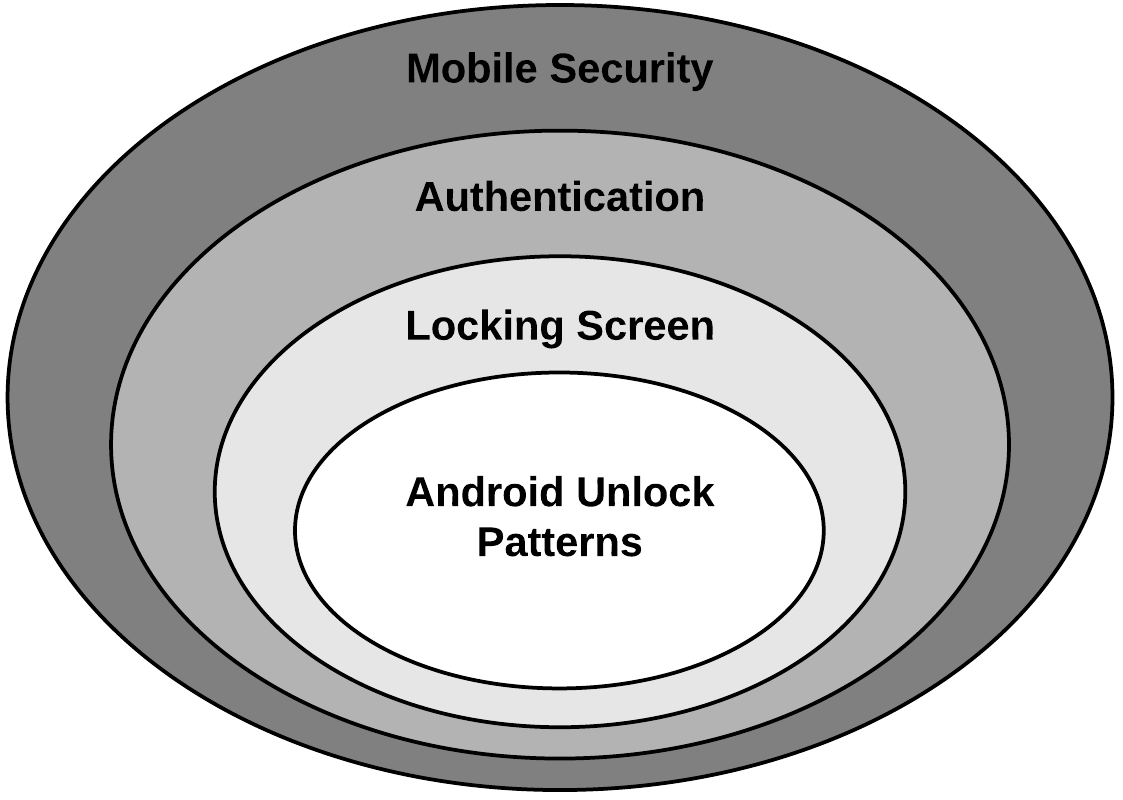
\includegraphics[scale=0.25]{pics/Fieldofstudy.png}
    \caption{Field of study}
    \end{figure}

    \section*{Keywords}  
    In the `field of study' I specified a specific scope in order to avoid to broad search space. 
    Inside each of the circles we can get more into details and create specific keywords that I will use in 
     the litterature search. 

    \begin{tabular}{ || l | l ||}
      \hline
      {\bf Mobile Security} & \\
      {\bf Locking Screen} &  \\
      {\bf Authentication} &  \\
      {\bf Android Unlock Patterns} & \\ 
      {\bf Psycology} & \\
      {\bf Graphical passwords} & \\
      \hline
    \end{tabular}
    \section*{Review Protocol}
